%Version 3.1 December 2024
\documentclass[pdflatex,sn-mathphys-num]{sn-jnl}

\usepackage{gensymb}
\usepackage{graphicx}
\usepackage{multirow}
\usepackage{amsmath,amssymb,amsfonts}
\usepackage{amsthm}
\usepackage{mathrsfs}
\usepackage[title]{appendix}
\usepackage{xcolor}
\usepackage{textcomp}
\usepackage{manyfoot}
\usepackage{booktabs}
\usepackage{longtable}
\usepackage{xurl}
\usepackage{algorithm}
\usepackage{algorithmicx}
\usepackage{algpseudocode}
\usepackage{listings}
\usepackage{tikz}
\usetikzlibrary{shapes,arrows.meta,positioning}
\lstset{breaklines=true,breakatwhitespace=false,columns=fullflexible}

\hypersetup{hypertexnames=false}
\raggedbottom

\begin{document}

\title[Empty Quarter Knowledge Base]{A formal knowledge base for amplicon sequencing data and geochemistry of the Rub' al Khali desert}

\author[1]{\fnm{Rund} \sur{Tawfiq}}
\author[1]{\fnm{Marwa} \sur{Abdelhakim}}
\author[2]{\fnm{Sulaiman M.} \sur{Alajel}}
\author[1]{\fnm{Mohammed} \sur{Alarawi}}
\author[3]{\fnm{Hind} \sur{Aldakhil}}
\author[1]{\fnm{Abderahmane} \sur{Derouiche}}
\author[4]{\fnm{Daniela I.} \sur{Drautz-Moses}}
\author[5]{\fnm{Michel} \sur{Dumontier}}
\author[6]{\fnm{Raik} \sur{Gr\"unberg}}
\author[1]{\fnm{Alejandra} \sur{Lopez-Velazquez}}
\author[7]{\fnm{Susana} \sur{Martinez Arbas}}
\author[1]{\fnm{Kexin} \sur{Niu}}
\author[1]{\fnm{Krishnakumar} \sur{Sivakumar}}
\author[8]{\fnm{Tiannyu} \sur{Wang}}
\author[4]{\fnm{Xiang} \sur{Zhao}}
\author[1]{\fnm{Jood} \sur{Zubair}}
\author[8]{\fnm{Magnus} \sur{Rueping}}
\author*[1]{\fnm{Robert} \sur{Hoehndorf}}\email{robert.hoehndorf@kaust.edu.sa}
%% ORCIDs received from co-authors (August 2026), for the submission system.
%% sn-jnl's \orcid{} macro needs Orcidlogo.eps, which is not in this project,
%% so they are kept as comments here.
%%   Daniela I. Drautz-Moses    0000-0002-3739-0917
%%   Susana Martinez Arbas      0000-0001-7309-8190
%%   Alejandra Lopez-Velazquez  0009-0001-2873-5311
%%   Xiang Zhao                 0009-0007-8662-9406
%%   Jood Zubair                0009-0005-9532-0801
%%   Abderahmane Derouiche      0000-0002-3241-1424
%%   Kexin Niu                  0000-0002-7302-0462
%%   Hind Aldakhil              0000-0001-9491-103X
%%   Mohammed Alarawi           0000-0001-8986-8209
%%   Rund Tawfiq                0000-0002-7052-573X  (ORCID registry, 6 Sep; to confirm)
%%   Marwa Abdelhakim           0000-0001-6816-2119  (ORCID registry, 6 Sep; to confirm)
%%   Michel Dumontier           0000-0003-4727-9435
%%   Raik Gr\"unberg             0000-0001-9532-6043
%%   Robert Hoehndorf           0000-0001-8149-5890


\affil[1]{\orgdiv{Bio-Ontology Research Group (BORG), Computer, Electrical and Mathematical Sciences and Engineering (CEMSE) Division}, \orgname{King Abdullah University of Science and Technology (KAUST)}, \orgaddress{\city{Thuwal}, \country{Saudi Arabia}}}
\affil[2]{\orgname{Ministry of Environment, Water and Agriculture}, \country{Saudi Arabia}}
\affil[3]{\orgdiv{National Livestock \& Fisheries Development Program (NLFDP)}, \orgname{Ministry of Environment, Water and Agriculture (MEWA)}, \orgaddress{\city{Riyadh}, \postcode{13413}, \country{Saudi Arabia}}}
\affil[4]{\orgdiv{Bioscience Core Lab}, \orgname{King Abdullah University of Science and Technology}, \orgaddress{\city{Thuwal}, \country{Saudi Arabia}}}
\affil[5]{\orgdiv{Institute of Data Science, Department of Advanced Computing Sciences, Faculty of Science and Engineering}, \orgname{Maastricht University}, \orgaddress{\city{Maastricht}, \country{The Netherlands}}}
\affil[6]{\orgdiv{Biomedical Sciences Division (BioMed)}, \orgname{King Abdullah University of Science and Technology (KAUST)}, \orgaddress{\city{Thuwal}, \country{Saudi Arabia}}}
\affil[7]{\orgname{NIUM}, \orgaddress{\city{Esch-sur-Alzette}, \country{Luxembourg}}}
\affil[8]{\orgdiv{Physical Science and Engineering (PSE) Division}, \orgname{King Abdullah University of Science and Technology (KAUST)}, \orgaddress{\city{Thuwal}, \country{Saudi Arabia}}}

\abstract{We collected soil and plant material during five campaigns across a 1,043~km transect of the Saudi Rub' al-Khali (Empty Quarter). The resource links 2,516 non-control specimen entries with laboratory processing and a canonical amplicon table of 1,271 profiles, of which 1,237 pass control and read-depth exclusions. Associated observations comprise 274 field environmental logs, 712 archived-soil pH measurements, 71 field X-ray fluorescence sessions, 725 laboratory X-ray fluorescence records and 3,234 site-month climate summaries. We represent sites, specimens, processes and measurement values in a modular RDF knowledge base using the Semanticscience Integrated Ontology and validated chemical, environmental and taxonomic references. Source ledgers preserve corrections, aliases and assay-specific provenance. Validation checks source reconciliation, measurement admission, identifier mappings, structural constraints and query outputs. The graph supports retrieval across these linked observations through a web portal and SPARQL endpoint. Versioned source tables, graph modules and workflow code support reuse, with raw-read availability and missing acquisition metadata identified as release dependencies.}

\keywords{Knowledge graph, Amplicon sequencing, Rub' al Khali, SIO, Semantic web}

\maketitle

\section{Background and summary}\label{intro}

The Rub' al-Khali (Empty Quarter) spans approximately 500,000 km$^2$
of the southern Arabian Peninsula \cite{mandaville_1986}. Its soils
experience large temperature fluctuations and irregular rainfall
\cite{nelli2024wind}, yet support diverse microbial communities
\cite{makhalanyane2015}. Repeated observations across soil compartments
and seasons provide a basis for studying these communities together
with their environmental conditions.

Previous Saudi Arabian surveys examined elevation gradients
\cite{yasir2015saudi}, rainfall responses across soil compartments
\cite{aslam2016rainfall}, and bulk and rhizosphere soils across regions
\cite{khan2020saudi}. Studies of desert plants further connected
microbial profiles with host-associated habitats \cite{eida2018plants}.
A repeated transect adds a specific data-management requirement:
each community profile must remain connected to its field specimen,
collection visit, laboratory processing and associated measurements.
Site identity alone is insufficient for temporal comparisons because
a site can have several visits and assays can use different field
replicates.

Multi-campaign resources such as Tara Oceans link campaign, station
and sampling-event registries to environmental and sequence data
\cite{taraoceans2015}. MIxS/MIMARKS specify contextual fields for
environmental sequence data \cite{mixs}, and STREAMS extends reporting
guidance for environmental microbiomes \cite{streams2025}. The National
Microbiome Data Collaborative uses persistent identifiers and shared
schemas to connect environmental microbiome data \cite{nmdc2026}.
Knowledge graphs such as KG-Microbe \cite{kgmicrobe2026} and
MetagenomicKG \cite{metagenomickg2026} organize taxonomic, functional and
environmental information across sources. We apply these principles
to the specimen and process provenance of a single landscape survey.

We collected soil and plant material during five campaigns
(2023--2025) along a 1,043~km transect across the Saudi Rub' al-Khali.
The catalogue contains 60 primary sites and 10 named locations.
A 2,550-row source ledger contains 2,516 non-control specimen rows.
The canonical amplicon table contains 1,271 profiles; the companion
ecology analysis retains 1,237 after control and read-depth exclusions.
Associated data comprise 274 field environmental logs, 712 admitted
archived-soil pH observations, 71 field XRF sessions, 725 laboratory
XRF records and monthly climate summaries. These counts describe
different observational units, whose links and coverage are documented
in the source ledgers.

We encoded sites, specimens, processes, qualities and measurement
values with the Semanticscience Integrated Ontology (SIO) \cite{sio}.
ChEBI \cite{chebi}, ENVO \cite{envo} and NCBI Taxonomy
\cite{ncbitaxon} provide chemical cross-references, environmental
classes and validated taxonomic identifiers. Original classifier
lineages and unresolved mappings retain their source provenance.
The resulting RDF modules support queries across these linked
observations.

Technical validation examines source reconciliation, measurement
admission, identifier mappings, structural constraints and executable
query examples. We report the scope of each check separately,
including the constructs and modules processed by ELK.
The portal at \url{https://rubalkhali.science/} exposes the graph
through site pages and a SPARQL endpoint. Data Records and Data
Availability identify the distributed artifacts and outstanding
release dependencies. The companion ecology manuscript reports the
community, environmental-association and functional analyses
\cite{ecology_companion}; this Data Descriptor documents their source
data, representation and reuse conditions.

\section{Methods}\label{methods}

\subsection{Study area and sampling design}

We conducted five sampling campaigns across the Rub' al-Khali along
a transect from the western escarpment (19.15\degree N, 45.17\degree
E) to the eastern border of Saudi Arabia with Oman (20.71\degree N,
54.73\degree E). The 60 ordered sampling sites yield a 1,043-km
cumulative path and lie 1,015~km apart end to end.
Figure~\ref{fig:transect} shows the site coordinates and altitude
profile. Cumulative distance sums great-circle distances between
successive sites, using an Earth radius of 6,371~km.

\begin{figure}[!htbp]
  \centering
  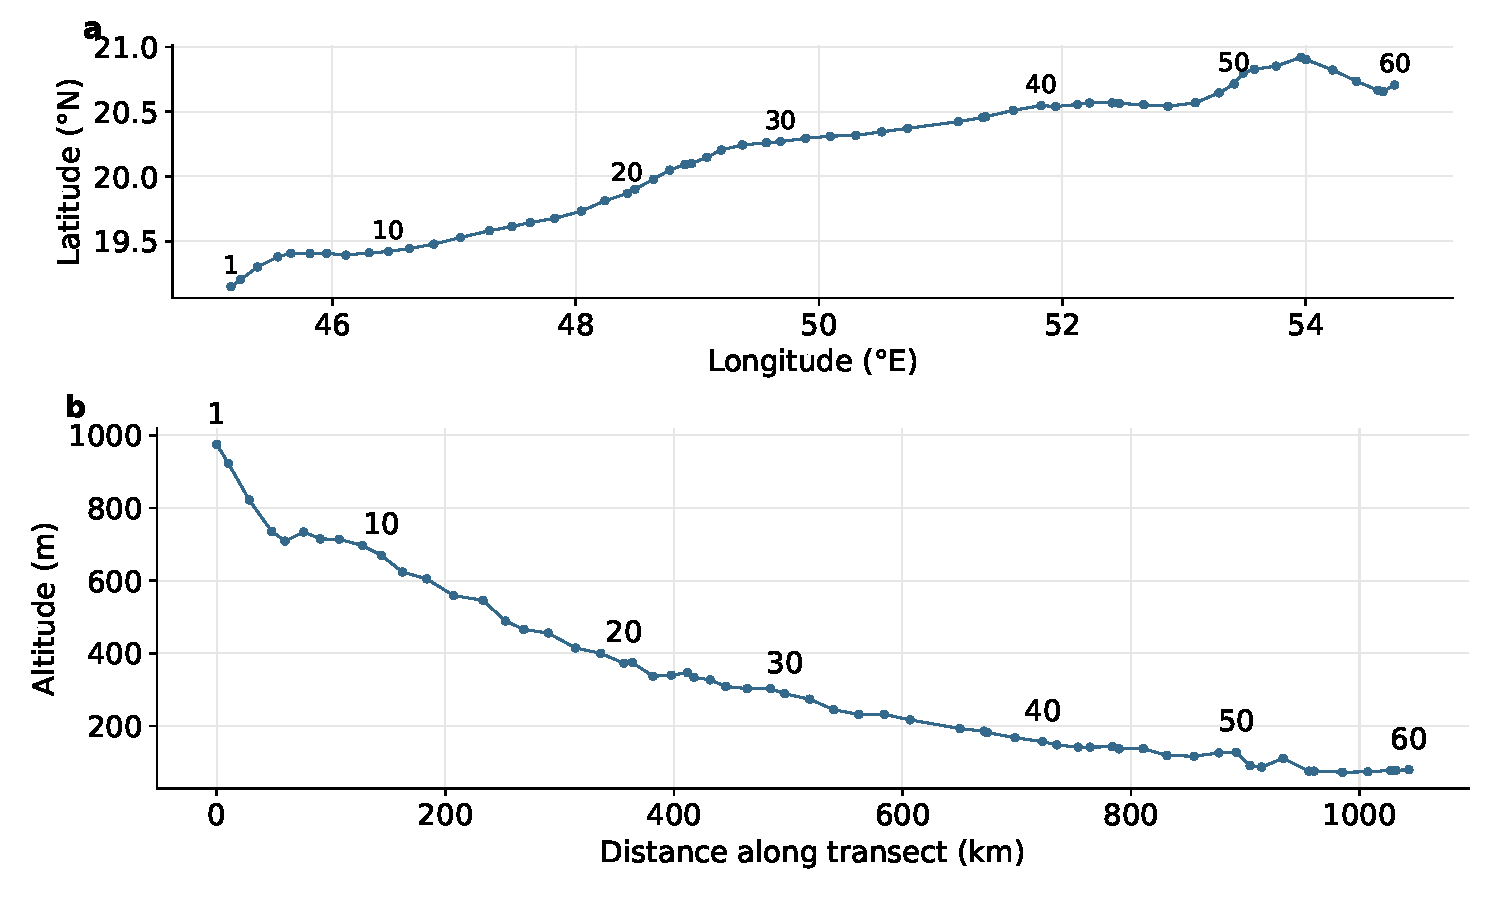
\includegraphics[width=\textwidth]{figures/transect/transect_altitude.pdf}
  \caption{Primary sampling transect across the Rub' al-Khali.
    Panel a shows the coordinates of sites 1--60; panel b shows their
    archived altitude values against cumulative great-circle distance
    in site order. Labels identify selected sites. Coordinates and
    altitude come from the versioned site-altitude table; the
    historical elevation source and vertical datum remain undocumented.}
  \label{fig:transect}
\end{figure}

The transect comprises 60 primary sampling sites at predetermined
coordinates and 10 named locations, including wells, a hot spring and
an oil-spill site. Trip~1 source identifiers 61--64 are aliases for four
named catalogue locations, established by coordinate matching.
The repeated-campaign analytical frame uses sites~1--60.
We preserve source sheets and apply the versioned correction ledger
to generate curated metadata.

To capture temporal variability, we conducted campaigns across
different seasons: late winter 2023 (Trip 1, 64 sites visited), summer
2023 (Trip 2, truncated to 8 sites due to extreme temperatures),
winter 2024 (Trip 3, 65 sites visited), summer 2024 (Trip 4, 60 sites
visited), and autumn 2025 (Trip 5, 62 sites visited). Field sheets provide temperature, atmospheric pressure and relative
humidity with campaign-specific availability. We summarize the
observational coverage in Table~\ref{tab:env_summary}. %, although the available measurements differ by campaign.
We acquired handheld field XRF measurements during Trip~5 and
laboratory XRF measurements of archived material from all five
campaigns. The curated environmental table retains 274 nonblank
source rows. Of these, 260 resolve to catalogue site visits and
generate 260 temperature, 187 pressure and 251 humidity values.
Fourteen auxiliary or revisit labels remain table-only pending
unambiguous site identification. The correction ledger assigns the
eight Trip~2 values 34.5--41.9 to temperature using their worksheet
context and the field note; pressure and humidity remain missing.
The Trip~5 site~40 humidity value of 194\% is retained in the source
ledger and excluded from the curated measurements.

\begin{table}[h]
  \centering
  \caption{Coverage of field environmental logs. Numeric identifiers, named
    locations and auxiliary observations retain separate source labels.}
  \label{tab:env_summary}
  \small
  \setlength{\tabcolsep}{3pt}
  \begin{tabular}{lllc}
    \toprule
    Campaign & Season & Field-log records & Measurements available \\
    \midrule
    Trip 1 & Late Winter 2023 & 1--60; 4 named; 15 auxiliary$^\ast$ & Temp, Press, Hum. \\
    Trip 2 & Summer 2023 & 1--8 & Temp. \\
    Trip 3 & Winter 2024 & 1--60; 5 named & Temp, Press, Hum. \\
    Trip 4 & Summer 2024 & 1--60 & Temp, Hum. \\
    Trip 5 & Autumn 2025 & 1--60; 2 named & Temp, Press, Hum. \\
    \bottomrule
  \end{tabular}
  \parbox{0.94\columnwidth}{\footnotesize $^\ast$The 15 records are appended
    to the legacy Trip~3 worksheet but are dated March 2023 in the
    original workbook and are curated as Trip~1 auxiliary/revisit
    observations.}
\end{table}



The sampling design targeted three soil
compartments: bulk surface soil, bulk subsurface soil
(5--10 cm depth, hereafter ``deep''), and subsurface soil collected
near roots (5--10 cm depth, hereafter ``root-adjacent''). 
The legacy class label Deep Soil Sample denotes the 5--10~cm
bulk compartment, called shallow-subsurface in the companion
ecology analysis \cite{ecology_companion}. We collected three
co-located field replicates per compartment using sterile tubes and
sterile plastic spoons. From Trip~2 onwards, three adjacent tubes
were taped or chained together for collection, so adjacent sampling
positions were separated by one external tube diameter. Trip~5
used larger tubes. Exact tube diameters, surface sampling depth
and distance from roots were unrecorded. These co-located
replicates share a site and compartment.
We preserved samples at $-20$\degree C in the field
using an Engel MR040F portable freezer. At the end of each campaign,
we transferred samples to an $-80$\degree C freezer in the laboratory.

The source ledger additionally contains 248 plant entries linked by
campaign, site and source identifier. Tissue type, host-identification
procedure, vouchers and plant-specific storage details are incomplete
in the archived protocol. These entries preserve plant provenance;
root-adjacent soil retains its own specimen identity.

\begin{table}[h]
\centering
\caption{Source-specimen coverage by campaign and soil compartment,
generated from \texttt{evidence/release/sample\_ledger.tsv}.
All catalogue sites are included; plant and control rows are excluded.
Columns count source rows eligible for specimen representation,
expected by the extract generator, linked to at least one run,
present in the ASV table and retained in the ecological analysis.
Repeated sequencing profiles can share one source-specimen row.}
\label{tab:sample_coverage}
\small
\setlength{\tabcolsep}{3pt}
% Generated by scripts/manuscript/generate_sample_coverage.py
\begin{tabular}{llrrrrr}
\toprule
Trip & Compartment & Specimens & Extract-linked & Run-linked & ASV table & Ecology \\
\midrule
1 & Subsurface & 192 & 184 & 111 & 110 & 108 \\
1 & Root-adjacent & 192 & 170 & 102 & 106 & 104 \\
1 & Surface & 192 & 185 & 108 & 114 & 113 \\
2 & Subsurface & 24 & 23 & 9 & 8 & 7 \\
2 & Root-adjacent & 24 & 18 & 13 & 13 & 11 \\
2 & Surface & 24 & 22 & 7 & 6 & 6 \\
3 & Subsurface & 180 & 180 & 141 & 141 & 141 \\
3 & Root-adjacent & 180 & 174 & 154 & 154 & 154 \\
3 & Surface & 180 & 180 & 156 & 155 & 155 \\
4 & Subsurface & 180 & 63 & 59 & 59 & 59 \\
4 & Root-adjacent & 180 & 60 & 58 & 58 & 58 \\
4 & Surface & 180 & 62 & 60 & 60 & 60 \\
5 & Subsurface & 180 & 93 & 57 & 55 & 55 \\
5 & Root-adjacent & 180 & 151 & 133 & 133 & 133 \\
5 & Surface & 180 & 82 & 30 & 29 & 29 \\
\bottomrule
\end{tabular}

\end{table}

\subsection{Laboratory controls}

Control coverage differed by campaign and processing stage
(Table~\ref{tab:controls}). Extraction blanks underwent the same
procedure as biological specimens. Trips~4--5 used one blank per
trip-specific extraction-day batch. Trips~1--3 used one blank per
extraction kit, and Trips~1--2 included shared extraction days.
The PowerSoil Pro control has a sequencing record
(\texttt{Extraction-Ctrl-Pro-Trip1}, library \texttt{M-25-0929});
the PowerSoil blank is present in laboratory records, with no matching
sequencing record located in the available sheets.

\begin{table}[h]
\centering
\caption{Control coverage relevant to the released amplicon data.
Detailed material and sequence occurrences are retained in the control
registry.}
\label{tab:controls}
\small
\setlength{\tabcolsep}{3pt}
\begin{tabular}{p{0.12\textwidth}p{0.25\textwidth}p{0.25\textwidth}p{0.26\textwidth}}
\toprule
Campaign & Extraction controls & PCR-stage negatives & Sequenced standards \\
\midrule
1 & Per-kit; Pro blank sequenced & Nuclease-free water & Identity unresolved \\
2 & Shared per-kit coverage & NTC-2 & Two purified-DNA standards \\
3 & Per-kit coverage & PCRCtrl, index 728 & Two whole-cell standards \\
4 & Six sequenced blanks; three unsequenced batches & PCR blank and NTC unsequenced & Amplification-positive control only \\
5 & 18 canonical blank profiles; 17 batch-linked & Six canonical NTC profiles & Field standard sequenced by shotgun \\
\bottomrule
\end{tabular}
\end{table}

The canonical table contains 18 Trip~5 extraction-blank profiles
(EB1--EB18) and six no-template PCR controls
(Negative1, Negative2, Negative4--Negative7). Seventeen extraction
blanks have confirmed batch links to 217 biological profiles.
The six Trip~4 extraction blanks (SEB, EB1--EB5) were sequenced on
a shared run and denoised separately with the same pipeline on
30~August 2026. Three of the nine Trip~4 extraction batches had
unsequenced blanks, leaving complete or partial coverage gaps at
28 sites. The corrected batch workbook supplies specimen-level
membership; the source-to-profile ledger also excludes unsequenced
S34Dr1 and S40PRr1. S40PRr1 failed three amplification attempts.
S34Dr1 yielded DNA but was probably missed during pooling.

No-template controls contained PCR reagents and molecular-grade water
in place of template DNA. Reagent-only PCR blanks contained neither
added water nor template. One reagent-only blank was prepared per
amplification plate. Most showed low or undetectable concentration
and adapter-dimer-dominated TapeStation profiles and were excluded
from sequencing. Trip~5 reagent-only blanks were lost during
handling, attributed to evaporation. Trip~4's PCR blank and NTC were
excluded because their index pairs conflicted with biological
libraries on the shared run. The Trips~1--3 control libraries were
sequenced on NovaSeq~6000 A01018 run~321, flowcell HVJY5DRX3, and
denoised with biological libraries in July 2025; they are distributed
separately from the canonical feature table. Re-denoising on
30~August 2026 supplied the control comparison in Technical Validation.

Positive standards were reserved for genus-recovery evaluation.
Trips~1--2 used the ZymoBIOMICS HMW DNA Standard D6322, introduced
at PCR; Trip~3 used the whole-cell D6300 Microbial Community Standard,
which also undergoes extraction. Trip~4 had a laboratory
amplification-positive control assessed by gel electrophoresis and
TapeStation, and Trip~5's field D6300 standard was sequenced by
shotgun metagenomics. Four sequenced standards from Trips~2--3
support the amplicon genus-recovery analysis. The Trip~1 FPosCtrl1
identity remains unresolved because its index and well disagree, so
it remains excluded.

D6322 contains seven bacterial genomes at 14\% genomic DNA each and
one yeast at 2\%; D6300 contains eight bacterial genomes at 12\% each
and two yeasts at 2\% each. These are manufacturer genomic-DNA mass
fractions. The recovery analysis compares expected and observed
bacterial genera, including unassigned reads and additional taxa.
Such departures can reflect processing contamination, amplification,
classification or index-assignment errors. The registry retains
intended materials, observed profiles and identity evidence separately.

\subsection{DNA extraction and sequencing}

Genomic DNA was extracted from 0.9--1.2~g of soil using either the
QIAGEN PowerLyzer PowerSoil Kit (catalogue no.\ 12855-50) or the QIAGEN
DNeasy PowerSoil Pro Kit (catalogue no.\ 47014). Both kits were used
in Trips~1--3: among the sequenced profiles, the sample ledger records
the PowerLyzer PowerSoil Kit for 77 Trip~1, 10 Trip~2 and 359 Trip~3
profiles (54 of the Trip~3 records name the MoBio PowerSoil kit) and
the DNeasy PowerSoil Pro Kit for 217 Trip~1, 11 Trip~2 and 87 Trip~3
profiles; 46 Trips~1--3 profiles have no recorded kit. The QIAcube
Connect was introduced for
routine extraction starting with Trip~4; samples from Trips~1--3 were
also processed using the QIAcube Connect when re-extraction was
required. The extraction method and re-extraction history were
recorded for each specimen when available.

Frozen soil samples were thawed on ice and processed immediately after
thawing. Before homogenization, samples were incubated at 65\degree C
for 10~min with agitation at 1,200~rpm, then homogenized using a
PowerLyzer 24 Homogenizer at 4,000~rpm for one 45-second cycle.
The remaining purification steps were performed either
manually or using a QIAcube Connect instrument, following the
manufacturer's protocol. DNA was eluted in 50~\textmu L of the elution
buffer supplied with the respective kit.

Extraction controls followed the campaign-specific scheme above.

Extracted DNA was quantified using the Qubit dsDNA High Sensitivity
assay, with fluorescence measured using a Varioskan LUX multimode
plate reader (Thermo Fisher Scientific). The project spreadsheet retains numerical extract concentrations. Progression to indexing and sequencing was
determined by an amplicon of the expected size after first-round PCR. DNA concentrations and processing information were recorded
in a central project spreadsheet. Extracted DNA was stored at
$-20$\degree C until PCR amplification.

The V3--V4 region of the bacterial 16S rRNA gene was amplified using
the Bakt\_341F (\texttt{CCTACGGGNGGCWGCAG}) and Bakt\_785R
(\texttt{GACTACHVGGGTATCTAATCC}) primers \cite{klindworth2013primers},
both carrying Illumina overhang adapters. First-round PCR was
performed using TaKaRa Ex Taq DNA Polymerase (catalogue no.\
RR001B). Each reaction had a total volume of 50~\textmu L and
contained 5~\textmu L of 10$\times$ buffer with Mg$^{2+}$,
4~\textmu L of dNTP mix (2.5~mM of each dNTP),
2~\textmu L of each 10~\textmu M primer stock, 0.25~\textmu L
of polymerase (5~U/\textmu L), 5~\textmu L of extracted DNA and 31.75~\textmu L
of nuclease-free water. The final primer concentration was
0.4~\textmu M per primer and 0.2~mM per dNTP, with 1.25~U
of polymerase per reaction. The PCR programme was: initial
denaturation at 95\degree C for 3~min; 35 cycles of 95\degree C for
10~s, 65\degree C for 30~s and 72\degree C for 1~min; and a final
extension at 75\degree C for 5~min.

First-round PCR products were assessed by electrophoresis on a 1\%
agarose gel. Samples showing an amplicon at the expected size of
approximately 500~bp were classified as passing and were then
indexed. Samples without a visible product were classified as failed;
these were re-amplified with 8~\textmu L and then 12~\textmu L of DNA,
with water reduced to 28.75~\textmu L and 24.75~\textmu L,
respectively. DNA input was set by volume because most extracts had low
or undetectable concentrations. Samples without a product after three
attempts were classified as failed; the earlier laboratory account also
documents re-extraction at the end of the workflow.

Dual indices and Illumina sequencing adapters were added in a
second-round PCR using the QIAGEN Multiplex PCR Kit (catalogue no.\
206143), following the Illumina 16S Metagenomic Sequencing Library
Preparation protocol \cite{illumina16S}: initial activation at
94\degree C for 15~min; 8 cycles of 94\degree C for 30~s, 55\degree C
for 30~s and 72\degree C for 30~s; final extension at 72\degree C for
5~min.

Indexed libraries were purified using Agencourt AMPure XP beads at a
0.8:1 bead-to-sample volume ratio,
quantified using the Qubit dsDNA High Sensitivity assay, and assessed
for fragment size using an Agilent 4200 TapeStation with the D5000
ScreenTape assay. Libraries were pooled by molarity calculated from
concentration and fragment size in the Core Lab pooling sheet.
Supplementary Section~S2 specifies the
pooling calculation and the remaining run-specific metadata gaps.
Amplicon pools were sequenced on an Illumina NovaSeq~6000 using
an SP flow cell with a 500-cycle reagent kit to generate
$2 \times 250$~bp
paired-end reads. Sample processing and library preparation were
performed in the PI's laboratory and sequencing was conducted at the
Bioscience Core Lab at KAUST.


\subsection{Sequencing data processing}

We processed raw amplicon reads with nf-core/ampliseq (v2.14.0)
\cite{nfcore, ampliseq}, applying the DADA2 algorithm \cite{dada2} for error
correction and denoising, and assigning taxonomy against the SILVA
database (v138.2) \cite{silva}. The submission records contain 1,268 run rows over 1,238 sample
identifiers, including 30 repeated identifiers. The feature-table
export separately contains 29 identifiers with nonidentical paired
columns; 28 retain both profiles after depth filtering. The source
ledger distinguishes submitted runs, physical libraries and analytical
profiles; the processing relationship of the paired export columns
remains unresolved.
This resulted in a canonical feature table of 351,472 amplicon sequence
variants (ASVs) prior to contaminant removal, covering samples from Trips~1--5 and 24 control samples.
Of its 1,271 profiles, 1,247 are biological; quality filtering excludes
the 24 control profiles and 10 biological profiles with fewer than
1,000 reads, leaving the 1,237 profiles used by the companion ecology
analysis. The complete table is distributed unfiltered. The reconstructed
input sheet and accession map are
\path{metadata/amplicon/combined_samplesheet_portable.csv} and
\path{metadata/amplicon/combined_samplesheet_accessions.tsv}.
The archived command specifies the Bakt\_341F/Bakt\_785R primers,
the NovaSeq option, DADA2 SILVA v138.2 assignment and skipped QIIME
steps; \path{metadata/amplicon/README.md} gives the full invocation
and resource configuration. The archived paired-read source sheets
identify all 1,271 canonical profiles: 1,013 occur in the July
sheet and 258 in the Trip~5 sheet. A further 33 July-sheet entries
fall outside the frozen feature table. The July sheet records
pipeline groups A and B. The profile-level reconciliation is
\path{metadata/amplicon/current_inventory/canonical_profile_read_inventory.tsv}.
The container digest, denoising parameters, physical run allocation
and export/merge provenance remain incomplete for exact table
regeneration.


We compared ASV prevalence in the 17 eligible Trip~5 extraction
blanks with prevalence in the 217 batch-linked biological profiles
\cite{fierer2025controls}. Presence means a read count greater than
zero. For each of the 351,472 ASVs, the one-sided Fisher test compares
present/absent profile counts in these two groups. ASVs absent from
all eligible blanks receive a score of one. The exploratory candidate
rule requires $p<0.1$ (uncorrected), presence in at least two blanks,
and higher prevalence in blanks than in biological profiles.
It identifies 351 candidates and applies their removal only to the
217 linked biological profiles. Prevalence is estimated across batches,
each represented by one blank; the canonical table remains unfiltered.

The threshold sensitivity table
(\path{evidence/control-audit/trip5_filter_sensitivity.tsv}) also
reports $p<0.01$ and $p<0.05$, yielding 221 and 300 candidates with
the two-blank rule. At $p<0.1$, requiring one or three blanks gives
12,051 or 175 candidates. This sensitivity documents the role of the
minimum-blank requirement. The control-recovery analysis separately
uses four standards from Trips~2--3.

The Trip~4 screen applies the same rule independently to six mapped
blanks and 95 biological profiles: one-sided Fisher $p<0.1$, presence
in at least two blanks and greater prevalence in blanks. It identifies
seven candidates, whose removal is restricted to these 95 profiles.
Replay with the corrected Trip~4 batch workbook reproduced the
combined 312-profile filtered matrix byte-for-byte after decompression.
The corrected source membership therefore preserves the archived
sensitivity-analysis input.

We inferred gene and pathway profiles from marker genes with PICRUSt2
v2.4.1 \cite{picrust2}. Two executions used the Trips~1--4 ampliseq
output and corrected Trip~5 output (330,830 ASVs). KO hidden-state
prediction used the PIC method, edge exponent 0.5 and seed 100.
EC/KO metagenome prediction required 100 reads; pathway inference
used the EC predictions. The command sequence and output identities
are documented in \path{metadata/functional/PICRUST2.md}.
The Trips~1--4 input sequences/table and their checksums remain
unavailable. The merged products contain 1,270 profile columns, whose
mapping is distributed with the functional tables.

\subsection{Taxonomy normalization and mapping}
\label{methods:taxonomy}


A taxonomic label can denote different taxa across databases and
releases, and a taxon can have several labels \cite{balvovciute2017silva}.
We therefore retain the original SILVA lineage alongside a validated
NCBI Taxonomy identifier or a lineage-scoped project identifier.
Taxonomic assignments come from SILVA v138.2 (Section~\ref{methods}), and we treat the original classifier lineage and ASV identifier as the primary evidence.
These assignments are seven rank fields (domain--species), and some are followed by a separate species assignment field and a numeric confidence. We assert the species from the ranked lineage and retain the additional species call in a provenance ledger.
We normalize the seven ordered rank 
fields by removing rank prefixes and representing empty and unclassified entries explicitly.

The mapping procedure evaluates the historical SILVA-to-NCBI candidates against a pinned NCBI Taxonomy release (the OBO Foundry NCBITaxon release \texttt{2025-03-13}, built from the NCBI
organismal taxonomy of 2025-03-01).
An identifier is retained only when it resolves, has a compatible rank and label or documented synonym, and its ancestor chain is compatible with all retained
higher-rank identifiers in that source lineage. A missing, ambiguous
or incompatible candidate is replaced by a deterministic project class
scoped to the complete truncated source lineage and rank. Each decision records the source
lineage and rank, candidate identifier, validation outcome, final
identifier and reason. The output mapping covers every 
lineage represented in both the taxonomy export and the
feature table; otherwise generation stops.

Existing project identifiers are retained only when all explicit
historical uses share one normalized rank, label and nearest explicit
parent context; a reused identifier that acquires more than one
corrected context is replaced in every affected use by contextual
classes. Each resulting class retains one rank, label and parent context. The mapping builder emits
corrected mappings, a decision ledger, a clean project taxonomy module
and a manifest containing input and output checksums, and the
abundance-ABox generator accepts only a passing, checksum-matched
manifest.

Queries retain the original SILVA lineage and independently validated
NCBI or project identifiers. The decision ledger reports rejected
candidates and their reasons. Algorithmic checks establish consistency
with the specified name, rank and ancestry rules; semantic mapping
accuracy requires a separately annotated validation sample.


\subsection{Shotgun-derived companion inputs}

The shotgun-derived companion inputs support downstream re-execution
from a genome catalogue and its annotations. Reproduction from raw
shotgun reads additionally requires the sequence accessions, genome
and proteome catalogues, and the assembly, binning, dereplication and
profiling workflows. These upstream inputs and parameters remain
missing from this package. We distribute
(i) 150 per-library CoverM \cite{coverm} genome-relative-abundance tables
(\path{metadata/metagenome/coverm_profiles.tar.gz}; one
column per shotgun library, in percent of reads, with the unmapped
fraction retained as its own row) and (ii) the eggNOG-mapper v2.1.12
annotation table \cite{eggnog}
(\path{metadata/metagenome/eq.emapper.annotations.gz}) of the
concatenated predicted proteome,
run on the KAUST Ibex cluster on 14 June 2026, from which a
990-genome by KEGG Orthology copy-number matrix is built for the
genomes present in both inputs. These files supply the genome-derived side of the companion
encoded-function comparison.

\subsection{PMA-treated aliquots}

The PMA dataset contains nine treated/untreated pairs from three
site-compartment groups at two Trip~5 campsites: C1 root-adjacent,
C2 root-adjacent and C2 surface soil. For each group, three soil
subsamples from one parent collection tube were prepared as separate
slurries. Each slurry was divided into treated and untreated aliquots,
giving three preparation pairs per parent tube.
Suspensions used PBS at pH~7.4 and a 1:10 mass-to-volume ratio.
Treated aliquots received 50~\textmu M PMAxx. Both treated and
untreated aliquots incubated for 10~min in darkness and were
illuminated at 450~nm for 35~min at 15--20~cm,
with rotation at 15-minute intervals. Samples were frozen at
$-20$\degree C; DNA was extracted from 860~\textmu L using the
PowerSoil Pro kit.

The paired marker-gene profiles describe treatment responses within
these three parent specimens under matched dark and light exposure.
% Marwa's 10 September 2026 clarification resolves parent identity:
% three separately prepared slurries per mother tube, one tube per group.

\subsection{Environmental and climate data}

We retrieved historical climate data from the Open-Meteo archive
endpoint \cite{openmeteo} for each sampling site using its geographic coordinates, yielding
12,936 monthly values: four variables over 49 months at 66 resolved
sites, or 3,234 site-month rows. The variables are temperature,
total precipitation, rainfall and relative humidity; annual summaries
are distributed separately. We ran two
separately configured acquisitions: the monthly product covers
1~January 2022 to 20~January 2026 and includes mean relative humidity,
whereas the daily product covers 1~January 2022 to 1~February 2026 and
reports temperature, total precipitation and rainfall.
January 2026 is a partial month in the monthly acquisition.
The frozen acquisition manifest
(\path{metadata/climate/climate_acquisition_frozen.json}) identifies
the query configuration and retained tables. Original response bodies,
retrieval timestamps and the historical model/product version remain
unavailable. Re-execution from these frozen tables preserves the
reported inputs; a new API request is a new acquisition.

Field researchers manually classified each site according to its biome (e.g., desert
biome) and specific environmental features (e.g., sand dune, saline pan, gravel, desert oasis). We subsequently mapped these
classifications to the Environment Ontology (ENVO) \cite{envo}.

\subsection{XRF acquisition, processing and reconciliation}\label{methods:xrf}

We acquired XRF data through two complementary workflows. During
Trip~5, field researchers used an Olympus Vanta VMR-XXX-G3-E
handheld analyser (serial 841307) for in-situ measurements. The source log contains 106 entries across
59 sites; 71 complete sessions at 58 sites were retained, and nine of
those sites have repeated complete sessions. The field log identifies measurement sessions and sites. Field and
laboratory observations are paired by site. Archived material from all five campaigns was
subsequently measured in the laboratory. The laboratory
inputs contain 547 selected sample records from Trips~1--4 and 178
from Trip~5 (725 records in total), and all 725 are used in the analyses.

All laboratory measurements used Fast Mode. The original Trip~5
workbooks specify Fast Screening-He8mm, helium and an 8~mm diameter
for all 178 canonical specimens. They retain element and oxide
reporting sections. For V4Dr3 and V18Dr3, the canonical table uses
the Fast Screening measurements; the two additional Best Detection
sheets remain source material. The Trips~1--4 consolidated workbook
preserves 28 export columns, while the exact gas and diameter
settings remain undocumented. Supplementary Section~S2
gives the acquisition audit and source selection.
The laboratory analyser model, measurement duration, tube settings,
sample preparation, concentration units and calibration records
remain incomplete. The concentration columns carry no unit
declaration. Percent formats occur in statistical-error columns,
and PPM labels occur in lower-limit-of-detection cells. We retain
instrument-reported magnitudes with undocumented concentration units.
At Site~4, field readings targeted soil and a second substrate described
as salt or oil; the source retains this unresolved substrate identity.

Both laboratory sources occasionally report the same formula more than once for one sample: the Trips~1--4 workbooks list a formula under several reporting sections (for example the element and oxide sections), and the Trip~5 workbook contains one sample (V14Dr1) with two readings. The two source-specific parsers resolve these repeats differently, taking the largest positive value for Trips~1--4 and the last reported row for Trip~5; these are processing rules adopted for the archived exports. The provenance audit reproduced all 13,390 reported Trips~1--4 cells and all 4,293 reported Trip~5 cells under these rules. In practice the two rules give the same value everywhere except three analyte cells (Al, Na and Si) of that one Trip~5 record, because repeated Trips~1--4 rows always carry identical values; a single rule would therefore change one of the 725 laboratory records, and the release discloses both source-specific policies.


The chemical audit evaluates 93 reporting channels against ChEBI
release 247 (3~December 2025) and the PubChem property snapshot of
23~July 2026 \cite{chebi,pubchem}. It retains 79 supported ChEBI
and 91 PubChem cross-references; unresolved channels have explicit
null identifiers. Checks cover identifier existence, labels, formula,
charge and element/oxide type. The P$_2$O$_5$ channel uses an
oxide-equivalent reporting basis linked to P$_4$O$_{10}$ by empirical
ratio. Light Elements remains an instrument-defined aggregate channel.

For a descriptive cross-workflow diagnostic, we took the median of repeated field sessions at each site and compared it with the Trip~5 Deep laboratory record at the 58 sites measured by both workflows.
The diagnostic estimates site-level rank agreement. Calibration would
require paired aliquots, documented units and reference materials.
Technical Validation reports the observed correlations.

\subsection{Archived-soil pH acquisition and admission}\label{methods:ph}

The frozen pH dataset is \texttt{EQ-PH-SHARED-v1.0.1}, with its
source manifest and admission ledger distributed under \path{metadata/ph/} and
\path{metadata/samples/ph/versions/EQ-PH-SHARED-v1.0.1/manifest.json}.
We measured archived dry soil after sieving below 2~mm. Each assay used an independent 1~g scoop suspended in 2.5~mL 0.01~M CaCl$_2$. Suspensions were mixed on a HulaMixer for 30~min and stood for 30~min at room temperature. We used an accumet AB315 meter with a Fisher Scientific accumet electrode (catalogue no.\ 13-620-112), and recorded the reading when the meter displayed its green stability indicator. The electrode was calibrated each morning at two points (pH 7 and 10), and we recorded the electrode slope and pH-10 buffer read-back for every session. Between samples, the electrode was rinsed along its full length with Milli-Q water, immersed in a separate container of Milli-Q water and dried by gently tapping with Kimwipes. A measurement was admitted only if its session was calibrated, the electrode slope was between 95\% and 102\%, and the read-back was within 0.1 pH units of nominal.

Admission additionally requires a numeric pH between 0 and 14 and an
accepted measurement date on or before 3~August 2026. Dates are read
from Excel date cells or parsed as ISO or day-first dates; unparseable
and post-cutoff dates remain quarantined. Threshold endpoints are
inclusive. Accepted measurements span 13~July to 2~August 2026.
The audit accounts for 1,168 workbook rows and admits 712 measurements. The remainder consisted of 356 rows without a measurement, 45 marked as depleted, 36 with ambiguous dates, and 19 numeric rows with incomplete quality control records.
Rows with unavailable values or incomplete admission evidence retain
their audit dispositions. We reconstructed 29 sessions from trip,
accepted date, electrode slope and pH-10 read-back.

All Trip~4 pH assays used archived field replicate~2. We reconciled
the specimen links for 155 admitted Trip~4 measurements against the
confirmed replicate-2 identifiers; one admitted measurement already
linked to replicate~2. The correction updates 620 RDF relations while
preserving all 712 admitted measurements, their numeric values and
the original workbook identifiers. The supported matching level with
community profiles is campaign, site and compartment.
The archived RDF protocol identifies an accumet AB315 with Probe~3
and automatic temperature compensation, and specifies mixing without
fine grinding.

\begin{table}[h]
\centering
\caption{Admitted archived-soil pH observations by campaign and
compartment. The specimen identifiers reflect the current admission
ledger; Trip~4 physical-replicate identity is discussed in the text.}
\label{tab:ph_coverage}
\small
\begin{tabular}{lrrrr}
\toprule
Campaign & Surface & Subsurface & Root-adjacent & Total \\
\midrule
1 & 52 & 56 & 49 & 157 \\
2 & 5 & 6 & 12 & 23 \\
3 & 54 & 50 & 52 & 156 \\
4 & 50 & 52 & 54 & 156 \\
5 & 30 & 57 & 133 & 220 \\
\midrule
Total & 191 & 221 & 300 & 712 \\
\bottomrule
\end{tabular}
\end{table}

\subsection{Knowledge representation}\label{ontology}

We represent the resource as a modular RDF knowledge base. The
terminology module (TBox) defines classes and relations in OWL
\cite{owl2}; the domain modules (ABoxes) describe sites, physical
specimens, processes and data products. Shared identifiers connect
these modules (Table~\ref{tab:modules}). SIO supplies the upper-level
classes and relations \cite{sio}. The terminology declares 333
classes (297 project classes and 36 referenced classes), 20 object
properties and 35 datatype properties. These counts apply to
declarations in the terminology module.

\subsubsection{Measurement and provenance}

We separate a measured quality from the information that quantifies
it. A temperature quality belongs to a site; a measurement process
produces a value for that quality. The value contains the numerical
reading and, where documented, its unit. Counts, dimensional
measurements and measurements with undocumented units use the
appropriate datatype and unit constraints in their assigned shapes.

Listing~\ref{lst:ttl_temp} illustrates this distinction for a field
temperature. The process belongs to a site visit, the visit targets
the site, and the measured quality is an attribute of that site.
The process-to-visit path supplies the observation context. SIO's
value-to-quality relation and its inverse support traversal in both
directions.

\begin{lstlisting}[caption={Field temperature and its visit provenance.},label={lst:ttl_temp},basicstyle=\ttfamily\scriptsize,frame=single]
@prefix rak: <https://rubalkhali.science/kb/RAK_> .
@prefix sio: <http://semanticscience.org/resource/SIO_> .
@prefix pato: <http://purl.obolibrary.org/obo/PATO_> .
@prefix uo: <http://purl.obolibrary.org/obo/UO_> .
@prefix xsd: <http://www.w3.org/2001/XMLSchema#> .

rak:P000001 a rak:0000006 ;
  sio:000068 rak:3000001 ;
  sio:000229 rak:4000001 .
rak:3000001 a rak:0000003 ;
  sio:000291 rak:1000001 .
rak:4000001 a rak:0000010 ;
  sio:000221 uo:0000027 ;
  rak:2000003 "20.7"^^xsd:double ;
  sio:000215 rak:5000001 .
rak:5000001 a pato:0000146 ;
  sio:000011 rak:1000001 ;
  sio:000216 rak:4000001 .
\end{lstlisting}

Sampling processes output material-sample collections. Collection
membership links each physical replicate to the sampling event;
the specimen's derivation edge also links it directly to its site.
A protocol is a reusable information specification, and a protocol
execution is a process. Extraction consumes soil and produces DNA;
library preparation consumes DNA and produces an amplicon library;
sequencing consumes the library and produces a digital FASTQ dataset.
Quality-control processes consume FASTQ datasets and produce
direction-specific metrics. Suppl. Sections~S1.2--S1.7 give the
corresponding formal patterns and graph examples.

Site annotations use existential restrictions to relate a site to
an ENVO biome or environmental feature. Such a restriction specifies
a filler of the named class. The source annotation ledger provides
the recorded assignment and its provenance.

Laboratory controls are occurrence-specific materials with
processing roles. A control-processing execution consumes the control,
realizes its role and belongs to a documented processing group.
Trips~4--5 use trip-specific extraction-day batches. Trips~1--3 use
per-kit controls, and Trips~1--2 include shared extraction days.
Occurrence-specific identifiers and the identity ledger distinguish
reused control labels. Confirmed, provisional, unresolved and
inapplicable dispositions retain their supporting evidence. The
D6300 whole-cell and D6322 purified-DNA standards enter the process
chain at extraction and PCR, respectively.

\subsubsection{Taxonomic and chemical observations}

For each profile, the taxonomy generator aggregates ASV counts at
seven ranks from domain to species, retaining the rank-truncated
classifier lineage and its validated NCBI or project identifier.
Each workflow produces fourteen datasets: read counts and relative
read abundance for each rank. The relative value divides the aggregated
count by the profile's total reads; explicit unclassified lineages
retain their contribution to that denominator. A taxon-rank entry adds a value and a
quality linked to shared dataset, workflow, taxon and FASTQ objects.
These links preserve the profile context during retrieval.
The taxon IRI is used as an individual in the abundance graph and as
a class in the mapping module. OWL~2 punning gives these uses separate
semantics: observation links identify the measured taxon, while
class-level axioms supply the reference ancestry. The generator
performs the rank aggregation explicitly.

XRF processes have several concentration-value outputs. A laboratory
process takes an archived specimen as input; a field process targets
a site and retains the instrument test identifier. The chemical
ledger supplies supported ChEBI and PubChem cross-references for
reporting channels, including oxide-equivalent channels. Unit
documentation and acquisition scope are described in
Section~\ref{methods:xrf}.

Archived-soil pH processes consume and target the assayed specimen,
produce a pH value linked to its acidity quality and belong to a
reconstructed measurement session. Field-replicate substitutions
require separate physical identities and an explicit campaign,
site and compartment matching level (Section~\ref{methods:ph}).

\subsubsection{OWL and RDF implementation}\label{subsec:owl_rdf}

Groovy scripts using OWL API v5.1.20 \cite{owlapi} generate the modules.
The modular organization separates domain data from shared terminology
\cite{cuencagrau2008modular}. OpenLink Virtuoso \cite{virtuoso}
provides RDF storage and SPARQL query execution.

KG v3.0.0 serves the asserted union. A separate reasoning workflow
uses the bundled rule program, v1.5.0, to compute consequences of a
specified set of positive RDF rules. These rules expand equivalent
classes and properties, subclass and subproperty hierarchies,
instance types, domains, resource-valued ranges, inverse and symmetric
properties, and transitive properties. The schema audit generates
rules for each nonempty finite property-chain pattern in the loaded
schema, including inverse operands. Additional rules introduce and
classify value restrictions, classify existential restrictions from
existing edges and typed fillers, propagate universal restrictions
to existing resource fillers, and handle intersections, union
membership and resource enumerations. All conclusions use existing
RDF terms. The schema audit lists the loaded imports and the
constructs outside this rule set.

The asserted graph contains the deduplicated union of the loaded
modules. Rules read this graph together with a separate inferred
graph and insert only conclusions absent from both. Each update
selects a bounded batch of distinct conclusions; each rule repeats
until its next batch adds zero triples. The complete schedule repeats
until every rule adds zero triples in one full pass. This stopping
criterion defines the least fixed point of the emitted rule program.
The instance-subclass rule is partitioned by instantiated named
classes, with a separate partition for anonymous classes. The class
inventory is refreshed each pass, so types introduced later in the
schedule enter subsequent passes.

The controller preserves the rule text, partition inventories,
per-batch additions, runtime versions and input identifiers.
Query truncation, SQL errors and exhaustion of the pass limit
terminate the run with a failure status. After convergence, separate
diagnostics test explicit disjoint-class and complement clashes,
membership in \texttt{owl:Nothing}, and incompatible laboratory-control
roles. These diagnostics and the finite rule set define the scope
of operational entailment validation.

\subsubsection{Structural constraints}\label{subsec:schema_def}

ShEx shapes \cite{shex} check selected nodes for required types,
properties, cardinalities and datatypes. The sampling-site shape
requires a site type, label and geometry predicate. Its unconstrained
geometry object checks presence; validation of the WKT datatype and
coordinate syntax is a separate requirement. Additional type
assertions are accepted independently of how they were obtained.

The sample shape requires a replicate type, a label, a source
identifier and an IRI-valued derivation edge. The DNA concentration
shape checks its numeric value, nanograms-per-microlitre unit and
quality/process links. The XRF-process shape requires a protocol,
one or more values and an input or target IRI. Checking the class of
that input or target requires a corresponding target shape or
scientific-invariant check. These open shapes admit predicates
outside their declared constraints; the negative fixtures test the
specific failures reported in Technical Validation.


\subsection{Schema validation}

We checked RDF structure using Shape
Expressions (ShEx) \cite{shex}. ShEx provides a formal structural
schema language that validates the presence, cardinality, and datatype
of RDF properties. We defined specific ShEx shapes for all core entity
types in the knowledge graph. These entity types include sampling
sites, soil samples, DNA extracts, sequencing datasets, measurements,
quality control records, laboratory control materials, control roles,
laboratory batches, control sequence occurrences, archived-soil pH
processes, values and sessions, and taxonomy mappings.

We integrated this schema validation into our deployment workflow
using a Shape Map. The Shape Map functions as a binding directive,
explicitly linking node selectors (e.g., all instances of the sampling
site class) to their respective ShEx shape definitions. The workflow
tests each newly generated segment of instance data against the
schema. It terminates the deployment if it detects missing mandatory
properties (e.g., GPS coordinates for a sampling site) or invalid
datatypes. Each passing test establishes conformance to the assigned shape's
specified constraints.
We implemented this validation using the Apache Jena ShEx library (v4.10.0) invoked from custom Groovy scripts.
The multi-gigabyte taxonomy ABox is excluded from this memory-bounded
ShEx run; the exact generated file is instead parsed in full with an
independent Turtle parser and checked by a streaming validator over
every classification process--dataset--quality--value relationship.

\subsection{Logical consistency (OWL reasoning)}

We ran ELK v0.4.3 \cite{elk} through OWL API v4.5.26, loading
the tractable modules into a merged ontology. This operational check
processes the constructs supported by ELK. The modules also contain
universal restrictions, inverse properties and other constructs
outside that support. An explicit OWL profile report and checked
projection are required to establish the logical scope of the result.
The run excludes the multi-gigabyte taxonomy ABox and large
reference modules. We report the loaded axioms and the return value
separately from structural validation in Technical Validation.

\subsection{Reproducible workflow}

The Nextflow entry point \texttt{main.nf} orchestrates module
generation, validation and manuscript-derived statistics. Local and
cluster profiles configure execution infrastructure. The versioned KG
release workflow regenerates the scientific modules, checks their
hashes against the frozen manifest, loads a fresh asserted database
and validates source-derived query results before switching the public
service.
Upstream sequence processing has its own samplesheets, workflow
parameters and environments.

The release manifests identify fixed source artifacts and generated
modules. Reproduction has three stages: downstream analyses from
curated inputs, generation of those inputs from primary records,
and replication of the field/laboratory measurements. The package's
workflow evidence covers the executed stages; missing upstream
sequence-processing inputs and acquisition metadata are stated in
their respective Methods subsections. A complete release requires a
fresh-checkout execution record, checksum comparisons and successful
main/supplement builds against the same inputs.

\section{Data records}\label{records}

The source and derived-data package contains graph modules, curated
tables, source and correction ledgers, validation evidence and workflow
code. The machine-readable manifest
\path{PRE_RELEASE_MANIFEST.tsv} identifies payload sizes, checksums,
categories and release/licence status. Separately retrieved bulk
payloads are listed in the bulk manifest. Data Availability reports
the current access routes and outstanding sequence-release gate.

KG v3.0.0 contains 45,706,977 asserted triples from 16 manifested
modules. The website distributes three versioned artifacts: the
scientific source package, the original RDF modules and the
deduplicated asserted graph in compressed N-Quads format.
The \href{https://rubalkhali.science/downloads/kg/3.0.0/manifest.json}{release manifest}
identifies their contents, sizes and checksums.

\subsection{Knowledge-graph modules}

The primary artifacts are the knowledge-graph modules, distributed as
RDF/XML and Turtle files and structured by data type
(Table~\ref{tab:modules}). The base ontology
(\texttt{rubalkhali.owl}) holds the project terminology. Domain modules
share site, specimen and process identifiers; the release also includes
the generated taxonomic vocabulary and four pinned reference ontologies.
These modules load together into an RDF store. Domain queries require the corresponding
shared terminology and linked site, specimen or process modules.

\begin{table}[h]
\centering
\caption{The 16 RDF modules included in KG v3.0.0.}
\label{tab:modules}
\small
\begin{tabular}{p{0.38\textwidth} p{0.54\textwidth}}
\toprule
\textbf{Module} & \textbf{Content} \\
\midrule
\texttt{rubalkhali.owl} & Base ontology (TBox) \\
\texttt{rubalkhali\_sites.owl} & Sampling sites with coordinates and biome annotations \\
\texttt{rubalkhali\_samples.owl} & Soil and plant specimen individuals with compartment types \\
\texttt{rubalkhali\_measurements.owl} & Field environmental measurements and climate records \\
\texttt{rubalkhali\_xrf.owl} & XRF measurement values from the field and laboratory workflows \\
\texttt{rubalkhali\_dna.owl} & DNA extracts with concentration data \\
\texttt{rubalkhali\_sra.owl} & Sequencing run records linked to ENA accessions \\
\texttt{rubalkhali\_qc.owl} & Sequencing quality metrics (GC content, duplicate rate, sequence counts) \\
\texttt{rubalkhali\_controls.ttl} & Laboratory-control materials, roles, batches and sequence occurrences \\
\path{rubalkhali_ph_eq_ph_shared_v1_0_1.ttl} & Archived-soil pH measurements, sessions and reconciled specimen links \\
\texttt{rubalkhali\_taxonomy\_abox.ttl} & Taxon observations over feature profiles \\
\texttt{ecosystem\_module.ttl} & Vocabulary supporting canonical taxonomic mappings \\
\texttt{sio.owl} & Semanticscience Integrated Ontology v1.59 \\
\texttt{envo.owl} & Environment Ontology, 20 October 2025 \\
\texttt{pato.owl} & Phenotype and Trait Ontology, 14 May 2025 \\
\texttt{uo.owl} & Units Ontology, 25 May 2023 \\
\bottomrule
\end{tabular}
\end{table}

\subsection{Tabular data products}

Alongside the graph, the deposit distributes the curated tabular data
products from which the modules are generated: the versioned source
ledger linking site and trip to specimen, extraction, library,
sequence run, quality-control decision and derived community; the
canonical Trips~1--5 amplicon feature table and its taxonomy mapping;
the correction and alias ledgers that record every deterministic
metadata repair without overwriting source values (the alias ledger
maps the 36 genuine Trip-1-only records of numeric sites 61--64 to the
four existing named site individuals); the curated field
environmental table; the field and laboratory XRF tables together with
the audited chemical-mapping ledger; and the versioned archived-soil
pH dataset \texttt{EQ-PH-SHARED-v1.0.1}. The canonical feature table
holds 1,271 profiles, of which the ecological analysis retains 1,237
(1,227 profiles from the primary frame of sites~1--60); the 34 excluded
profiles are the 24 controls, nine biological profiles
below the declared 1,000-read ecological threshold and one additional
\texttt{T1Dr1} run with 934 reads. The four derived
companion-analysis inputs are distributed as records for downstream
statistical re-execution: the paired PMA
table (\path{metadata/relic-dna/PMA_ASV_table.tsv}; 18 analytical
columns from nine aliquot pairs, PMA-treated and untreated, with
controls kept separately), the 150 CoverM profiles
(\path{metadata/metagenome/coverm_profiles.tar.gz}), the eggNOG
annotations (\path{metadata/metagenome/eq.emapper.annotations.gz})
behind the 990-genome analytical subset, and the measured-function
input archive (\path{metadata/metagenome/measured_function_inputs.tar.gz})
with the six exact source tables of the genome-derived versus PICRUSt2
comparison. These are fixed inputs for downstream analyses. Methods identifies
the additional raw reads, upstream workflows and acquisition metadata
needed for end-to-end reproduction.

\subsection{Validation schemas, queries and evidence}

The deposit includes the artifacts needed to re-validate the resource:
the ShEx shapes that define the structural contract for each entity
family, the positive and negative structural fixtures, the archived
competency SPARQL queries, and the machine-readable evidence bundles
(reconciliation summaries, audit tables, validation records and
checksum manifests) produced by the release workflow. A companion data
dictionary (\path{metadata/DATA_DICTIONARY.tsv}) records the field
names, data types, units, missing-value conventions and definitions
for the curated canonical tabular records. Quantities carry units only
where a unit is documented at the source: environmental source tables
retain degrees Celsius, hectopascals (millibars) and percent relative
humidity; in the graph, pressure magnitudes are
multiplied by 100 and asserted in pascals (\texttt{obo:UO\_0000110}),
climate
records use degrees Celsius and millimetres, and DNA concentrations
are in nanograms per microlitre. XRF values are instrument-reported magnitudes with undocumented
concentration units.

The manifests and data dictionary provide the versioned file-level
inventory. The final archival dataset citation remains a release gate
(Section~\ref{data_availability}).

\section{Technical validation}\label{valid}

Technical validation separates source reconciliation and measurement
checks from structural constraints, executable queries and the
operational ELK check. The evidence bundles identify the input
snapshot and checks executed.

\subsection{Assay validation}

The PowerSoil Pro extraction-control profile contained 1,165 ASVs,
with 84\% of reads assigned to ASVs shared with biological profiles.
Its nearest canonical profile was 46Dr1, with Bray--Curtis
dissimilarity 0.39. We excluded this control from the contaminant
screen. A library-order test compared nearby library numbers with
different-site pairs matched by geographic-distance decile and
compartment, using 999 library-order permutations. The Trip~1 and
Trip~3 Bray--Curtis contrasts were $-0.003$ ($p=0.15$) and
$+0.007$ ($p=1.0$), respectively. These contrasts summarize the
tested preparation-order association.

For XRF, the source audit reproduces 13,390 Trips~1--4 and 4,293
Trip~5 reported cells under their stated selection rules.
Repeated field sessions were reduced to site medians and paired
with the Trip~5 subsurface laboratory observation at 58 sites.
Among 12 analytes with positive values in both workflows at more
than 10 paired sites, the median Spearman correlation was 0.21
(range $-0.40$ to 0.48;
\path{evidence/xrf_audit/xrf_field_lab_agreement.tsv}).
This diagnostic describes site-level rank agreement among the
retained positive pairs.

\subsection{Competency questions and SPARQL queries}

Competency questions define the intended retrieval tasks
(Table~\ref{tab:cq}). The archived query workload covers site,
geochemical, molecular-provenance and taxonomic data. The
Site~10 XRF query has an archived 46-row result. Source-derived
expected result tuples also specify the complete 48-observation
genus profile for run \texttt{ERR16061083},
360-row environment--taxon join, 70 site coordinates and six
PCR no-template control roles. The release validator compares full
result multisets, preserving duplicate rows and requiring exact
identifiers. Numeric comparisons use absolute and relative
tolerances of $10^{-12}$; coordinate comparisons use an absolute
tolerance of $10^{-10}$ degrees. The 26 checks cover the printed
queries across direct and application-mediated transports, default
and explicit datasets, and a 20-row taxonomic API result.

Six additional checks verify the advertised asserted-only dataset,
the rejection of unavailable query modes, the absence of unreleased
graphs, the default graph cardinality and all 712 pH
process--specimen links against the reconciled source module.
Fourteen protocol checks cover dataset selection, read-only access
and preservation of RDF terms across the supported graph and
SELECT serializations. Browser validation executes all nine portal
examples and checks the three versioned download links. Full HTTP
downloads verify artifact sizes and checksums; the complete asserted
N-Quads export is parsed and checked for its graph context and triple
count. All checks passed on the candidate and public service. The
\href{https://rubalkhali.science/downloads/kg/3.0.0/post-deployment-validation.json}{public validation report}
binds these results to the release manifest.
Separate structural tests cover additional module types.

\begin{table}[h]
\centering
\caption{Competency questions defining the retrieval workload.}
\label{tab:cq}
\small
\begin{tabular}{p{0.08\textwidth} p{0.84\textwidth}}
\toprule
\textbf{ID} & \textbf{Competency question} \\
\midrule
CQ1 & What are the XRF analyte concentrations measured at a given sampling site? \\
CQ2 & Which sampling sites are recorded, and what are their GPS coordinates? \\
CQ3 & Which biome and environmental features are assigned to each sampling site? \\
CQ4 & What are the instrument-reported Light Elements values across the XRF measurements? \\
CQ5 & Which DNA extraction records (extract, concentration, protocol) exist for a given sample? \\
CQ6 & What is the full provenance chain from a soil sample to its sequencing run? \\
CQ7 & What are the complete genus-level read counts and relative read abundance for run \texttt{ERR16061083}? \\
\bottomrule
\end{tabular}
\end{table}

We show several example SPARQL queries. Listing~\ref{lst:sparql_xrf}
retrieves XRF measurements for a specific site, requiring traversal of
the measurement process, quality, and value entities.

\begin{lstlisting}[caption={SPARQL query to retrieve field XRF
    measurements for Site 10. The query starts from the field-XRF
    measuring processes whose target is the site and walks to the
    individual analyte concentrations.},
  label={lst:sparql_xrf}, basicstyle=\ttfamily\scriptsize,
  frame=single]
PREFIX rak: <https://rubalkhali.science/kb/RAK_>
PREFIX sio: <http://semanticscience.org/resource/SIO_>
PREFIX rdfs: <http://www.w3.org/2000/01/rdf-schema#>

SELECT ?processLabel ?siteLabel ?analyte ?concentration
WHERE {
  ?process a rak:0000025 ;
           rdfs:label ?processLabel ;
           sio:000291 ?site ;
           sio:000229 ?value .
  FILTER(CONTAINS(LCASE(STR(?processLabel)), "field xrf"))
  ?site rdfs:label ?siteLabel .
  FILTER(?siteLabel = "Site 10")
  ?value sio:000215 ?quality ;
         rak:2000012 ?concentration .
  ?quality a ?qualityClass .
  ?qualityClass rdfs:label ?analyte .
  FILTER(?qualityClass != rak:0000032)
}
ORDER BY ?processLabel ?analyte
\end{lstlisting}

The query selects field-XRF processes targeting Site~10, then
retrieves each output and its analyte quality. It returns one row
per process/analyte combination, excluding the aggregate Light
Elements channel. The concentration units are undocumented.

The release workflow executes this exact query
(\path{sparql/field_xrf_site10.rq}) against the checksummed base, site
and XRF modules and requires the fixed expected cardinality of
46 analyte-value rows; it returned exactly 46 rows for Site~10,
24 from field process Test~5847 and 22 from Test~5848, and the result
table and validation record are archived under
\path{evidence/competency-query/}.
This execution checks the archived query's cardinality; release
validation also requires comparison of stable identifiers and values
with the expected table.

Listing~\ref{lst:sparql_taxon} retrieves the complete genus profile for
run \texttt{ERR16061083},
joining across bioinformatic workflows, FASTQ datasets, and taxon
observations.

\begin{lstlisting}[caption={Complete genus-level profile for run ERR16061083, ordered by descending read count and lineage.},label={lst:sparql_taxon},basicstyle=\ttfamily\scriptsize,frame=single]
PREFIX rak: <https://rubalkhali.science/kb/RAK_>
PREFIX sio: <http://semanticscience.org/resource/SIO_>
PREFIX rdfs: <http://www.w3.org/2000/01/rdf-schema#>
PREFIX xsd: <http://www.w3.org/2001/XMLSchema#>

SELECT ?proc ?fastq ?runLabel ?lineage ?taxon ?taxonLabel
       ?count ?relativeAbundance
WHERE {
  VALUES ?runLabel { "FASTQ dataset for ERR16061083" }
  ?proc a rak:0000071 ;
        sio:000230 ?fastq ;
        sio:000229 ?dsAbs, ?dsRel .
  ?fastq rdfs:label ?runLabel .
  ?dsAbs a rak:0000074 ; rdfs:label ?absLabel ;
         sio:000059 ?valAbs .
  ?dsRel a rak:0000075 ; rdfs:label ?relLabel ;
         sio:000059 ?valRel .
  FILTER(STRENDS(STR(?absLabel), "(Genus)"))
  FILTER(STRENDS(STR(?relLabel), "(Genus)"))
  ?valAbs rak:2000026 ?count ;
          rak:2000025 ?lineage ;
          sio:000215 ?qualAbs .
  ?valRel rak:2000020 ?relativeAbundance ;
          rak:2000025 ?lineage ;
          sio:000215 ?qualRel .
  ?qualAbs sio:000011 ?taxon, ?fastq .
  ?qualRel sio:000011 ?taxon, ?fastq .
  ?taxon rdfs:label ?taxonLabel .
  FILTER(?taxon != ?fastq)
}
ORDER BY ?runLabel DESC(xsd:double(?count)) ?lineage ?proc
\end{lstlisting}

The query binds both count and relative-abundance values to the same
workflow, source FASTQ dataset, taxon and classifier lineage. Dataset
labels currently encode rank through the suffix \texttt{(Genus)}.
The query uses that emitted convention explicitly and returns all
48 observations for the named run. The source-derived expected table
contains the complete profile, including each classifier lineage.
The separate \path{scripts/release/kg/taxonomy_all_runs.rq} retrieves
all runs from a locally loaded snapshot. That unrestricted export
is a long-running operation. The environmental example below additionally binds
field temperature and specimen collection to the same site visit.

\begin{lstlisting}[caption={SPARQL query to retrieve Pseudomonas relative abundance at sites with high temperature.}, label={lst:sparql_env_tax}, basicstyle=\ttfamily\scriptsize, frame=single]
PREFIX rak: <https://rubalkhali.science/kb/RAK_>
PREFIX sio: <http://semanticscience.org/resource/SIO_>
PREFIX pato: <http://purl.obolibrary.org/obo/PATO_>
PREFIX ncbitaxon: <http://purl.obolibrary.org/obo/NCBITaxon_>
PREFIX rdfs: <http://www.w3.org/2000/01/rdf-schema#>
SELECT ?visit ?visitLabel ?site ?siteLabel ?sample ?fastq
       ?temperatureProcess ?tempVal ?temp ?lineage ?relAbundance
WHERE {
  ?visit a rak:0000003 ; rdfs:label ?visitLabel ;
         sio:000291 ?site .
  ?site rdfs:label ?siteLabel .
  ?temperatureProcess sio:000068 ?visit ;
                      sio:000229 ?tempVal .
  ?tempVal rak:2000003 ?temp ; sio:000215 ?tempQual .
  ?tempQual a pato:0000146 ; sio:000011 ?site .
  FILTER(?temp > 35.0)
  ?sampling a rak:0000024 ; sio:000068 ?visit ;
            sio:000291 ?site ; sio:000229 ?collection .
  ?collection sio:000059 ?sample .
  ?ext sio:000230 ?sample ; sio:000229 ?dna .
  ?libPrep a rak:0000065 ; sio:000230 ?dna ;
           sio:000229 ?lib .
  ?seq a rak:0000066 ; sio:000230 ?lib ;
       sio:000229 ?fastq .
  ?bioinf a rak:0000071 ; sio:000230 ?fastq ;
          sio:000229 ?dsRel .
  ?dsRel a rak:0000075 ; rdfs:label ?datasetLabel ;
         sio:000059 ?valRel .
  FILTER(STRENDS(STR(?datasetLabel), "(Genus)"))
  ?valRel rak:2000020 ?relAbundance ;
          rak:2000025 ?lineage ; sio:000215 ?qualRel .
  ?qualRel sio:000011 ncbitaxon:286, ?fastq .
}
ORDER BY ?visit ?sample ?fastq ?tempVal ?lineage
\end{lstlisting}

Each result retains the collection visit, specimen, sequence dataset,
temperature observation and genus lineage. A site's visits are joined
through their process provenance. This provides an environmental
temperature associated with the collection visit of each returned
microbial profile.

Regression fixtures execute both queries on deliberately confusable
inputs. The taxonomy fixture assigns the same genus different
abundances in two profiles and adds a species-rank observation; the
query returns exactly the two matching genus observations. The visit
fixture gives one site two visits at 40 and 20\degree C; the
temperature-filtered query returns only the specimen collected during
the 40\degree C visit. These tests check the implemented joins;
release-level validation additionally requires expected result tables
for the complete modules.

\subsection{Source reconciliation and measurement validation}

The archived evidence workflow produced a row-level sample ledger and
reconciliation summaries for specimens, extracts, libraries, runs and
community profiles. The 2,516 eligible source rows reconcile exactly
to 2,516 generated sample individuals; the 1,647 extraction-eligible
rows reconcile to 1,647 DNA extracts; and 1,242 resolved sequence rows
reconcile to 1,242 amplicon libraries and 1,242 FASTQ datasets. A
site-alias gate independently matches each Trip~1 numeric identifier
61--64 to a named catalogue individual by exact coordinates and
rejects coordinate or IRI disagreement, accounting for all 36 affected
source rows.

The environmental-metadata gate reproduced 274 nonblank source records
and verified all 24 exact-cell correction-ledger dispositions against
the corresponding raw cells. All retained field temperatures,
pressures and relative humidities fell within their declared physical
ranges; the unresolved Trip~5 site~40 value of 194\% was preserved in
the ledger but is absent from both the curated table and the
environmental RDF module. The XRF provenance audit reproduced all
13,390 reported Trips~1--4 cells under the maximum-positive rule and
all 4,293 reported Trip~5 cells under the last-reported rule, with no
mismatched reported cells, and verified that the canonical laboratory
input comprises all 725 processed records. An independent
chemical-identifier gate checked all 93 instrument channels against
the pinned ChEBI release 247 and the checksummed PubChem snapshot of
23 July 2026 (Section~\ref{methods:xrf}); all
rows passed the declared rules, with explicit nulls for the aggregate
LE channel and unsupported oxides. The pH reconciliation accounts for 1,168 workbook rows and
reproduces the five admission dispositions in
Section~\ref{methods:ph}. The string-based join associates each
admitted row with a specimen identifier; the Trip~4 physical-replicate
correction requires the separate provenance reconciliation described
there.

\subsection{ShEx schema validation}

The archived ShEx run used the shapes described in
Section~\ref{subsec:schema_def}. Its tractable modules passed their
assigned shapes. The pH module was
validated separately over all 712 measurement processes, values and
acidity qualities and all 29 sessions, and the laboratory-control
module passed its shape and scientific-invariant checks. Four negative
fixtures each alter one constraint: missing site coordinates, an invalid
value datatype, reversed value-to-quality direction, or an XRF process
with neither input nor target. The released shapes reject all four
fixtures. The
multi-gigabyte taxonomy ABox remains outside this memory-bounded run;
it is instead parsed in full by an independent Turtle parser and
scanned by a streaming structural validator, which accounted for
44,528,482 triples in 5,953,690 subject blocks with zero structural
violations. This checks full-file syntax and the generator's declared structural
relationships. The separate listing validator checks printed Turtle
against the modules available for that run. Taxonomy and external
reference checks require the corresponding pinned payloads.

\subsection{Logical consistency}

The 9 September validation loaded 781,044 asserted axioms from eleven
ontology IRIs and ELK returned \texttt{true} for its consistency check.
The checked union included the ecosystem, pH and laboratory-control
modules. It excluded the taxonomy ABox and large reference modules;
imported axioms were not added to the asserted union, and class-hierarchy
precomputation was omitted. An import-order regression confirmed that
modules loaded through imports and then encountered explicitly retain
their asserted axioms exactly once.

The generated assertions include \texttt{xsd:double} literals, placing
the asserted graph outside OWL~2~EL's datatype restrictions
\cite{owl2profiles}. An OWLAPI profile diagnostic on the tractable
asserted core found 40,482 illegal-datarange occurrences, including
40,481 uses of \texttt{xsd:double}. Diagnostics caused by missing
import declarations were recorded separately. ELK's operational
result describes the asserted union under the constructs processed
by this ELK configuration.

Validation of the separate finite-rule implementation uses synthetic examples for long
hierarchies, transitive cycles, both project property-chain lengths,
restriction and intersection classification, and PCR-control ancestry.
The tests compare bounded, class-partitioned execution with an
unbounded reference closure and check recovery from an interrupted
run. Release-specific checks compare the complete control-role
inventory with its source, retrieve consequences of the measurement
chains and require the inferred graph to be disjoint from the
asserted graph. Completion requires the zero-addition pass specified
in Section~\ref{subsec:owl_rdf}, followed by the explicit clash
diagnostics.

The separate label gate merged 800,026 triples and confirmed exactly
one label for each of 106,833 labelled \texttt{RAK\_} subjects.
Current logs, input hashes and validator sources are preserved under
\path{evidence/final-validation-20260909/}; the earlier run remains
under \path{evidence/semantic-validation/}.

\subsection{Compute-time metrics}\label{sec:compute_metrics}

Table~\ref{tab:compute} preserves development timings for a
nine-ABox snapshot. The original benchmark lacks the complete
hardware, repetition and cache information needed for a portable
performance comparison. It differs from the current module set.
The query timings range from 5~ms to a timeout above 300~s.

\begin{table}[h]
\centering
\caption{Historical development timings; these describe an earlier
  nine-ABox snapshot.}
\label{tab:compute}
\small
\begin{tabular}{lr}
\toprule
\textbf{Step} & \textbf{Time} \\
\midrule
RDF module loading (Virtuoso, 9 ABox files)  & 140\,s \\
Selected rule expansion (3 passes)           & 114\,min \\
ELK check (historical benchmark)           & 1.6\,s \\
CQ1 -- XRF measurements, Site 10            & 23\,ms \\
CQ2 -- Sampling sites + GPS                 & 5\,ms \\
CQ3 -- Biomes per site                      & 5\,ms \\
CQ4 -- Light Elements reported values       & 8\,ms \\
CQ5 -- DNA extraction records               & 1{,}342\,ms \\
CQ6 -- Provenance chain                     & 255\,ms \\
CQ7 -- Taxonomic composition                & $>$300\,s \\
\bottomrule
\end{tabular}
\end{table}

CQ7 exceeded the five-minute timeout in that benchmark. A subsequent
global 100-row preview and an equivalent two-branch formulation also
exceeded 300~s on the idle release candidate. These runs are archived
with their exact queries. The current CQ7 demonstrates a complete
profile for a named run; its acceptance test compares all observations
with an independently derived source table. Performance measurements
must identify the query and graph snapshot used.

\subsection{Portal access}

The portal (\url{https://rubalkhali.science/}) retrieves data through
backend SPARQL queries and renders site and specimen views. This is
an access interface. Independent validation compares query results
with source-derived expected values; a user study would additionally
measure task completion, errors and usability.

\subsection{Identifiers and reuse metadata}

Each named entity has a project-domain IRI. The manifest identifies
payload files, and the data dictionary specifies curated fields,
units and missing-value conventions. RDF provenance links travel
with the modules and support reuse through SIO, ENVO, ChEBI, PATO,
UO and validated taxonomic identifiers \cite{fair}.

The public endpoint provides read access to the deployed graph.
A fixed archival package additionally requires a versioned deposit,
verified payload access, a persistence policy and explicit licences
for project data, code and externally sourced material. Data
Availability identifies the remaining sequence-release gate.

\section{Usage notes}\label{usage}

The portal at \url{https://rubalkhali.science/} provides site pages and
a SPARQL editor. The endpoint
\url{https://rubalkhali.science/sparql} accepts SPARQL~1.1 queries.
For a local, low-memory example, load the base, site and XRF modules
listed in Table~\ref{tab:modules} and execute
\path{sparql/field_xrf_site10.rq}. The archived Site~10 result contains
46 rows; compare both the returned process/analyte identifiers and
their values with \path{evidence/competency-query/}. Taxonomic
queries additionally require the taxonomy ABox and its mapping
dependencies. The named-run example retrieves the complete genus
profile for \texttt{ERR16061083}. For all-run exports, execute
\path{scripts/release/kg/taxonomy_all_runs.rq} on a locally loaded
snapshot and allow for a long-running join. The release's \path{REPRODUCE.md} describes payload
retrieval, checksums, environments and workflow commands.

\subsection{Choosing observations for reuse}

Use specimen, collection-visit and assay identifiers when joining
observations. The primary repeated-campaign frame comprises sites
1--60; the source identifiers 61--64 refer to four named catalogue
locations sampled in Trip~1. Several feature profiles share a source
specimen identifier. Analyses should group these profiles by their
documented specimen and processing relationships.

The control registry distinguishes assay, processing stage,
extraction group and identity evidence. The Trip~5 candidate screen
uses 17 extraction blanks linked to 217 biological profiles and
identifies 351 ASVs. The canonical feature table retains these ASVs;
the companion sensitivity analysis applies their removal to the linked
profiles. Trip~4 has six separately denoised extraction blanks and
three batches with unsequenced blanks, leaving complete or partial
coverage gaps at 28 sites. Concentration measurements exist in the
source records; any concentration-based screen requires a matched
specimen--extraction--measurement ledger. Four Trips~2--3 standards
support genus-recovery evaluation. Trips~4--5 have extraction controls
but no sequenced 16S positive-standard profiles.

Archived-soil pH describes specimens measured in CaCl$_2$ under the
admission rules of Section~\ref{methods:ph}. Coverage varies by
campaign and compartment. All Trip~4 assays used archived field
replicate~2. Their supported comparison with community profiles is at
campaign, site and compartment level. The versioned reconciliation
links measurements to the confirmed specimens as described in Methods.

Field and laboratory XRF observations have separate acquisition
provenance and undocumented concentration units. The released values
support within-workflow descriptive comparisons; cross-workflow
calibration requires documented units, paired aliquots and reference
materials. Site~4 field readings include different substrates, so a
site-level summary combines that local heterogeneity with instrument
repeatability.

The PMA table contains three site-compartment groups at two campsites.
Each group has one parent collection tube, from which three separate
slurries supplied treated/untreated pairs. Descriptive paired summaries
retain this preparation structure and compare dye treatment under
matched dark and light exposure.

\subsection{Versioning and supported operations}

The deposited source and checksum manifests identify the inputs used
to generate each module. Preserve these files when reproducing a
reported result. Rebuilding against a newer external ontology requires
identifier and mapping validation, followed by regeneration of the
affected modules and query results. The repository changelog records
source corrections and superseded artifacts.

KG v3.0.0 serves the asserted graph at
\url{https://rubalkhali.science/graph/asserted/3.0.0}.
This graph is the default dataset for portal and SPARQL queries.
Explicit \texttt{FROM}, \texttt{FROM NAMED} and SPARQL protocol
dataset parameters select the dataset for an individual request.
The service evaluates stored assertions directly and rejects
unavailable query modes.

The bundled finite-rule implementation supports the separate
reasoning workflow described in Section~\ref{subsec:owl_rdf}.
Publication of its output requires completion and validation of that
workflow. Changes to released artifacts require a new semantic version.

For reproduction, retain the source package, module manifest,
loader provenance and checksums together. The release instructions
specify the pinned generation environment and coordinate-preserving
import adapter. The asserted N-Quads provides the released union;
the source package regenerates all 16 original module hashes.
Local module loading provides access to fixed inputs independently
of the portal's deployed version. Analyses requiring additional OWL
consequences need a reasoner and validation workload suited to those
constructs.

\section{Data availability}\label{data_availability}

The project uses ENA umbrella study \texttt{PRJEB104209}; its submitted
amplicon run records are associated with \texttt{PRJEB106069}. On
10~September 2026, the anonymous ENA read-run file report for
\texttt{PRJEB106069} returned no public run/file rows. Release of the
raw reads or a complete anonymous reviewer download remains required.
The source and derived-data package is maintained at
\url{https://github.com/bio-ontology-research-group/empty-quarter-ecology-data}.
Its manifests distinguish included files, separately retrieved bulk
payloads and unresolved release gates. KG v3.0.0 and its source package
are available through the versioned website downloads. The broader
dataset's archival accession, sequence access and project-data licence
remain separate publication requirements.

\section{Code availability}\label{code}

The web application and ontology-development code are available at
\url{https://github.com/bio-ontology-research-group/empty-quarter}.
The data repository
\url{https://github.com/bio-ontology-research-group/empty-quarter-ecology-data}
contains the manuscript sources, RDF generators, metadata and
\texttt{main.nf} workflow. RDF generation uses Groovy scripts with
OWL API v5.1.20 \cite{owlapi}; the ELK validation wrapper uses
OWL API v4.5.26. The repository supplies execution profiles, workflow
tests, a pinned Conda recipe and a hash-locked Python environment.


% Author-approved acknowledgements remain to be supplied.

\section*{Funding}
Susana Martinez Arbas was supported by the Fonds National de la Recherche (FNR), Luxembourg
(Project Ref.\ 18047750).
% Additional author-confirmed funding remains to be supplied.

% Author-confirmed CRediT contributions remain to be supplied.

\section*{Competing interests}
The authors declare no competing interests.

\bibliography{sn-bibliography}

\end{document}
